\section{Cahier des charges}

\subsection{Définitions}

\begin{itemize}[label=\textbullet]
    \item \textbf{Micro-capsules}: petit cylindres en verre fermés des deux côtés (borosilicate). \\ 
    Diamètre extérieur = 2,8 ± 0,05 mm; \\
    Diamètre intérieur = 2,5 ± 0,05 mm; \\
    Longueur = 10 mm

    \item \textbf{Réacteurs}: Flacons à sertir en verre dimension: 11 mm, 12 x 32, 2 ml 
    
    \item \textbf{Bloc de réaction}: Plaques « Para-Dox » avec 48 positions, Gen II, pour flacons 12 x 32
\end{itemize}

\subsection{Analyse du besoin}

\begin{figure}[H]
    \centering
    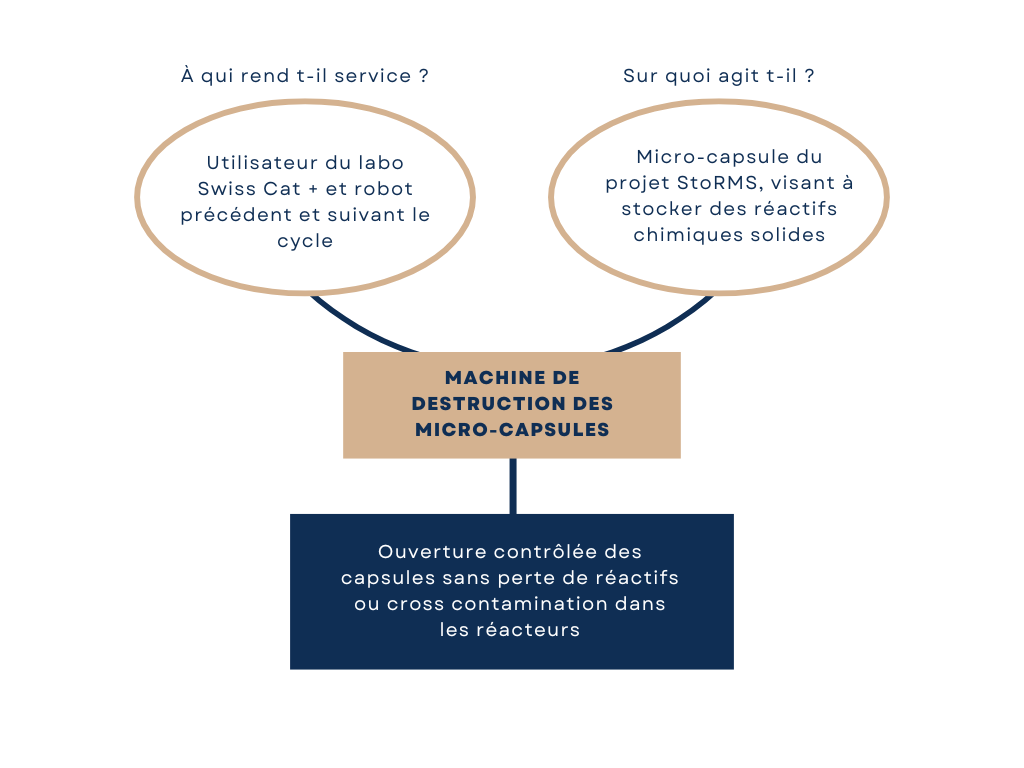
\includegraphics[width=15cm]{Images/Illustrations/CDH/Bete a corne.png}
    \label{fig:beteacorne}
    \caption{Diagramme bête à corne}
\end{figure}

\begin{table}[H]
    \centering
    \begin{tabular}{
    >{\columncolor[HTML]{FFFFFF}}l |
    >{\columncolor[HTML]{FFFFFF}}l }
    {\color[HTML]{000000} \textbf{\#}} & {\color[HTML]{000000} \textbf{Besoin}}           \\ \hline
    {\color[HTML]{000000} \textbf{1}} & {\color[HTML]{000000} Ouvrir des micro-capsules} \\ \hline
    {\color[HTML]{000000} \textbf{2}} & {\color[HTML]{000000} } \\ \hline
    {\color[HTML]{000000} \textbf{}}  & {\color[HTML]{000000} } \\ \hline
    \end{tabular}
    \caption{Liste des besoins du système}
    \label{tab:besoin}
    \end{table}

\subsection{Fonctions et exigences du système}
\subsubsection{Fonctions de services}

Les fonctions de services correspondes aux exigences principales du produits (réflexions basé sur cahier des charges du projet multi 2024 \cite{projmulti2024}).


\begin{table}[H]
    \centering
    \begin{tabular}{
    >{\columncolor[HTML]{FFFFFF}}l 
    >{\columncolor[HTML]{FFFFFF}}l |
    >{\columncolor[HTML]{FFFFFF}}l 
    >{\columncolor[HTML]{FFFFFF}}l }
    \multicolumn{2}{l|}{\cellcolor[HTML]{FFFFFF}{\color[HTML]{000000} \textbf{Fonctions de service}}} &
      \multicolumn{2}{l}{\cellcolor[HTML]{FFFFFF}{\color[HTML]{000000} \textbf{Exigences}}} \\ \hline
    \multicolumn{1}{l|}{\cellcolor[HTML]{FFFFFF}{\color[HTML]{000000} \textbf{FS 1}}} &
      {\color[HTML]{000000} \begin{tabular}[c]{@{}l@{}}Doit être en mesure \\ de détruire une micro-capsule\end{tabular}} &
      \multicolumn{1}{l|}{\cellcolor[HTML]{FFFFFF}{\color[HTML]{000000} \textbf{E 1}}} &
      {\color[HTML]{000000} \begin{tabular}[c]{@{}l@{}}Libération totale du réactif \\ (débris de verres inclus)\end{tabular}} \\ \hline
    \multicolumn{1}{l|}{\cellcolor[HTML]{FFFFFF}{\color[HTML]{000000} \textbf{FS 2}}} &
      {\color[HTML]{000000} \begin{tabular}[c]{@{}l@{}}Doit être en capable \\ de répéter la tâche\end{tabular}} &
      \multicolumn{1}{l|}{\cellcolor[HTML]{FFFFFF}{\color[HTML]{000000} \textbf{E 2}}} &
      \cellcolor[HTML]{FFFFFF}{\color[HTML]{000000} \begin{tabular}[c]{@{}l@{}}Répétabilité de la tâche \\ 48 fois par plaque\end{tabular}} \\ \hline
    \multicolumn{1}{l|}{\cellcolor[HTML]{FFFFFF}{\color[HTML]{000000} \textbf{FS 3}}} &
      {\color[HTML]{000000} } &
      \multicolumn{1}{l|}{\cellcolor[HTML]{FFFFFF}{\color[HTML]{000000} \textbf{E 3}}} &
      {\color[HTML]{000000} }
    \end{tabular}
    \caption{Fonctions de service}
    \label{tab:fctservice}
    \end{table}

\subsubsection{Fonctions technique}



\subsubsection{Fonctions de contraintes}








